\documentclass{article}

\usepackage{a4wide}
\usepackage[utf8]{inputenc}
\usepackage[T1]{fontenc}
\usepackage[french]{babel}
\usepackage[babel=true]{csquotes} % guillemets français
\usepackage{graphicx}
\graphicspath{{Images/}}
\usepackage{color}
\usepackage{hyperref}
\hypersetup{colorlinks,linkcolor=,urlcolor=blue}

\usepackage{amsmath}
\usepackage{amssymb}


\title{Rapport de projet de jeu avec accéléromètre}
\author{\'Thomas Lenepveu, M1 informatique}
\date{\today}

\begin{document}

\maketitle % pour écrire le titre


%% Le résumé:
\begin{abstract}
  Dans ce beau rapport, je vous donne quelques exemples
  de commandes \LaTeX.
\end{abstract}

\section{Une section}
\label{section:hello} % pour faire référence à la section ailleurs (\ref{...} voir plus bas)

Hello World!

\subsection{Une sous-section}
D'abord, une liste à \textbf{puces}:
\begin{itemize}
\item la documentation de \textit{Swing}~\cite{swingDoc}
  est bien écrite,
\item celle de \textit{Tkinter}~\cite{tkinterDoc} aussi!
\end{itemize}
% \cite{...} permet de faire référence à des éléments de la
% bibliographie.

\`A présent, une liste numérotée:
\begin{enumerate}
\item premier item
\item second item
\end{enumerate}

\subsection{Une autre sous-section}
Pour écrire du code, on peut par exemple utiliser l'environnement
\textit{verbatim}:
\begin{verbatim}
public class Main {
   public static void main(String[] args) {
      System.out.println("Hello World!");
   }
}
\end{verbatim}

\section{Une autre section}

% \ref{...} permet de faire référence à un élément défini
% ailleurs dans le document (voir \label{...} plus haut).
Contrairement à la section~\ref{section:hello},
moi je dis: \textit{Coucou!}

\subsection{Une sous-section}
Voici une belle image:
\begin{center}
  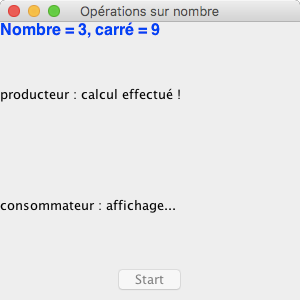
\includegraphics[scale=0.5]{exo3_1_1.png}
\end{center}



%%% La bibliographie:
\bibliographystyle{plain}
\bibliography{ma_biblio}

\end{document}
